\documentclass[a4paper, amsfonts, amssymb, amsmath, reprint, showkeys, nofootinbib ,twoside]{revtex4-2}
\usepackage[english]{babel}
\usepackage[utf8]{inputenc}
\usepackage[colorinlistoftodos, color=green!40, prependcaption]{todonotes}
\usepackage{amsthm}
\usepackage{mathtools}
\usepackage{physics}
\usepackage{xcolor}
\usepackage{graphicx}
\usepackage[left=23mm,right=13mm,top=35mm,columnsep=15pt]{geometry} 
\usepackage{adjustbox}
\usepackage{placeins}
\usepackage[T1]{fontenc}
\usepackage{lipsum}
\usepackage{amsmath}
\usepackage{amssymb}
\usepackage{braket} 
\usepackage{csquotes} 
\usepackage{booktabs}

\newcommand{\Hs}[1]{\mathcal H_{#1}}
\newcommand{\bd}[1]{\hat b^\dagger_{#1}}
\newcommand{\bb}[1]{\hat b_{#1}}
\newcommand{\nn}[1]{\hat n_{#1}}
\newcommand{\cre}[1]{\hat\beta^\dagger_{#1}}
\newcommand{\ann}[1]{\hat\beta_{#1}}
\newcommand{\cfree}[1]{\hat\beta^{(0)\dagger}_{#1}}


\usepackage[pdftex, pdftitle={Article}, pdfauthor={Author}]{hyperref} % Para enlaces en el PDF


%\setlength{\marginparwidth}{2.5cm}
%\bibliographystyle{apsrev4-1} 
\begin{document}
\title{Wave guides as an analogous system of 1D optical lattice for anyons}

\author{Ronaldo Navarro Ambriz}
    \email[Correspondence email address: ]{ron@estudiantes.unam.fisi}% Correo asociado 
    \affiliation{Instituto de Física, Universidad Nacional Autónoma de México, Ciudad de México, México} 
\author{Santiago Francisco Caballero Benítez}
    \email[Correspondence email address: ]{scaballero@fisica.unam.mx}% Correo asociado 
    \affiliation{Instituto de Física, Universidad Nacional Autónoma de México, Ciudad de México, México}

\date{\today} % Se puede cambiar o quitar, se usara para parte de llevar un registro 

\begin{abstract}
In this work we provide an analytical framework for describing the propagation of a quantum walk along an 1d optical lattice using the analogy of light in waveguide arrays, considering an infinite case for the waveguides, translating to the anyons systems the results from perturbative theory  allows to propose an external potential to recreate anyonic behavior in waveguides offering a feasible treatment into the propagation dynamics in these systems, and comparing the result with an non perturbative solution and a numerical solution via exact diagonalization of the Hamiltonian. 
\end{abstract}

\keywords{anyons, quantum matter, ultracold atoms, waveguides}


\maketitle

%\section*{Acknowledgements} \label{sec:acknowledgements}
    \lipsum[8]
\section{Introduction} 
Los anyones son ... 
\section{Theoretical Model} 
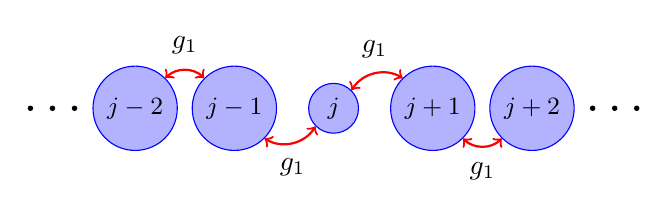
\begin{tikzpicture}[scale=0.7]
  % --- Define parameters ---
  \def\spacing{1.8} % Horizontal spacing between circles
  \def\ballradius{1.05} % Radius of the circles

  % --- Draw the chain ---
  % Dots on the left
  \foreach \x in {-5.5, -5.1, -4.7}
    \fill[black] (\x, 0) circle (0.05);

  % Simplified blue circles
  \foreach \j/\label in {-2/{j-2}, -1/{j-1}, 0/{j}, 1/{j+1}, 2/{j+2}} {
    \node[circle, draw=blue, fill=blue!30, minimum size=\ballradius*0.5cm, font=\small] (N\j) at (\j*\spacing, 0) {$\label$};
  }

  % Dots on the right
  \foreach \x in {4.7, 5.1, 5.5}
    \fill[black] (\x, 0) circle (0.05);

  % Red solid arrows for coupling
  \draw[<->, red, thick] (N-2) to[bend left=45] node[above=2pt, black] {$g_1$} (N-1);
  \draw[<->, red, thick] (N-1) to[bend right=45] node[below=2pt, black] {$g_1$} (N0);
  \draw[<->, red, thick] (N0) to[bend left=45] node[above=2pt, black] {$g_1$} (N1);
  \draw[<->, red, thick] (N1) to[bend right=45] node[below=2pt, black] {$g_1$} (N2);
\end{tikzpicture} 
Para las guías de onda:
\begin{itemize}
    \item Una guía de onda pose un indice de refracción en el otro núcleo, rodeado por otro de menor indice $n_1 < n_2$
    \item Para una única guía de onda, los modos admitidos están dados por sus características físicas. 
    \item Un arreglo de guías de onda, el acoplamiento permitirá la transferencia entre los elementos del arreglo.
\end{itemize} 
From an infinite waveguides array with homogeneous optical single mode waveguides and equally spaced along z-axis. This is described by the
following differential equation \cite{Jones1965Coupling}	
\begin{align}\label{EqEner}
    i \frac{dE_j(z)}{dz} = g_1 (E_{j-1} + E_{j+1}), \quad j = -\infty, \dots, \infty,
\end{align}
From this 
\begin{align}
     i \frac{d|\psi(z)\rangle}{dz} = \hat{H}|\psi(z)\rangle, \quad \hat{H} = g_1 \left( \hat{V}_\infty + \hat{V}_\infty^\dagger \right),
\end{align} 
where the operators $\hat{V}_\infty$ and $\hat{V}^\dagger_\infty$ are the infinite counterparts of the London-Susskind–Glogower operators
\cite{London1926, Susskind1964}, defined as
\begin{align}
      \hat{V}_\infty = \sum_{n=-\infty}^{\infty} |n\rangle \langle n+1|, 
\quad \hat{V}_\infty^\dagger = \sum_{n=-\infty}^{\infty} |n+1\rangle \langle n|, 
\end{align}
For an analytical solution we need to satisfy in our Hilbert space the following conditions for the LSG operator
\begin{align*}
    \left[\hat{V}_\infty, \hat{V}_\infty^\dagger\right] &= 0, \qquad \hat{V}_\infty \hat{V}_\infty^\dagger = \hat{I},
\end{align*}
In this framework the initial state is a photon in the $n$ site of an infinite array of waveguides $\ket{\psi(0)} = \ket{n_0}$,:
\[
\ket{\psi_{n_0}(z)} = \exp\left[-g_1 z \left(i\hat{V}_\infty^\dagger - \frac{1}{i\hat{V}_\infty^\dagger}\right)\right] \ket{n_0}.
\]
Donde podemos identificar la función generadora de las funciones Bessel, para obtener
\[
\ket{\psi_{n_0}(z)} = \sum_{n=-\infty}^{\infty} J_n(-2g_1 z)i^n \hat{V}_\infty^{\dagger n} \ket{n_0}.
\] 
para este modelo podemos hacer una analogía con un modelo de bosones en una red óptica partiendo del operador $\hat{V}_\infty$ y la evolución será escrita en función del tiempo:
\begin{align}
\hat{V}_\infty = \sum_{j=-\infty}^{\infty} \hat{b}_j^\dagger  \hat{b}_{j+1}, \quad \hat{V}_\infty^\dagger = \sum_{j=-\infty}^{\infty} \hat{b}_{j+1}^\dagger \hat{b}_{j} ,
\end{align}
Rewriting the Hamiltonian as 
\begin{equation}\label{NewHamiBos}
\hat{H} = -J \sum_{j=-\infty}^\infty \left( \hat{b}_j^\dagger  \hat{b}_{j+1} + \hat{b}_{j+1}^\dagger \hat{b}_{j}  \right)
\end{equation} 
The operator $\hat{V}^{\dagger n}_\infty$ is equivalent of create a particle in $n$ site in the framework of optical lattices for a subspace of one particle per site:
\begin{equation}
\hat{V}^{\dagger n}_\infty |1_0\rangle = \hat{b}^\dagger_n |0\rangle, 
\end{equation}	
Obtaining the dynamics for a particle in $0$-site 
\begin{equation} 
\ket{\psi_{0}(t)} = \sum_{n=-\infty}^{\infty} J_n(2 J t)i^n \hat{b}_n^{\dagger	} \ket{0}.
\end{equation} 
\subsection{One body observables for free bosons} 
We could obtain a rich dynamics for $n$-particle systems working with a Heisenberg representation for the one-body operators (Appendix~\ref{ap:pass}). With the dimensionless time and the free propagator
\begin{equation}\label{eq:Gn}
\tau\equiv 2Jt,\qquad G_n(\tau)\equiv i^{n}J_n(\tau)=i^{|n|}J_{|n|}(\tau),
\end{equation}
the bosonic operators evolve as $\hat b_j(t)=\sum_m G_{j-m}(\tau)\,\hat b_m$ and $\hat b^\dagger_j(t)=\sum_m G^*_{j-m}(\tau)\,\hat b^\dagger_m$. It is useful to build the one-body density matrix $\rho_{ij}(t)\equiv\langle\hat b_i^\dagger(t)\hat b_j(t)\rangle$ is then
\begin{equation}\label{eq:rhofree}
\rho_{ij}(t)=\sum_{m,m'}G^*_{i-m}(\tau)\,G_{j-m'}(\tau)\,\rho_{mm'}(0).
\end{equation}
The density is $\langle\hat n_j\rangle=\rho_{jj}$. For initial states without one-body coherences, i. e. $\rho_{mm'}(0)=\delta_{mm'}\langle\hat n_m(0)\rangle$ for Fock states, it reduces to
\begin{equation}\label{eq:nfree}
\langle \hat{n}_j(t) \rangle = \sum_{m} J^2_{j-m}(2Jt)\, \langle \hat{n}_m(0) \rangle .
\end{equation}
Each bond $(j,j+1)$ is characterized by its kinetic energy and its particle current, defined for anyons in Eqs.~(\ref{eq:Kj}) and (\ref{eq:Jj}); for bosons($\theta=0$),
\begin{align}
\hat{\mathbf K}_j&=-J\big(\hat b_j^\dagger\hat b_{j+1}+\hat b_{j+1}^\dagger\hat b_j\big),\\
\hat{\mathbf J}_j&=iJ\big(\hat b_{j+1}^\dagger\hat b_j-\hat b_j^\dagger\hat b_{j+1}\big),
\end{align}
with $\langle\hat{\mathbf K}_j\rangle=-2J\,\mathrm{Re}\,\rho_{j,j+1}$ and $\langle\hat{\mathbf J}_j\rangle=2J\,\mathrm{Im}\,\rho_{j,j+1}$. For coherence-free initial states, $G^*_{j-m}G_{j+1-m}=iJ_{j-m}J_{j+1-m}$ is purely imaginary, so
\begin{align}
\langle\hat{\mathbf K}_j(t)\rangle&=0,\label{eq:Kfree}\\
\langle\hat{\mathbf J}_j(t)\rangle&=2J\sum_m J_{j-m}(2Jt)\,J_{j+1-m}(2Jt)\,\langle\hat n_m(0)\rangle.\label{eq:Jfree}
\end{align}
%
%also: 
%\begin{equation} 
%\textbf{J} = \textit{i} J \sum_{i=1}^M \left(e^{-\textit{i} \theta\hat{n}_i}  \hat{b}_{i+1}^\dagger\hat{b}_i -   \hat{b}_{i}^\dagger\hat{b}_{i+1} e^{\textit{i} \theta\hat{n}_i} \right)
%\end{equation}
%\begin{equation} 
%\textbf{T} = J \sum_{i=1}^M \left(e^{-\textit{i}\theta\hat{n}_i}  \hat{b}_{i+1}^\dagger\hat{b}_i +   \hat{b}_{i}^\dagger\hat{b}_{i+1} e^{\textit{i}\theta\hat{n}_i} \right)
%\end{equation}
%\[ 
%\mathrm{S}(q) = \sum_{l=0}^M |\mathrm{J}_l ( -2Jt)|^2 - \sum_{l, m=0}^M e^{\mathrm{iq}(l-m)} |\mathrm{J}_l ( -2Jt)|^2  |\mathrm{J}_m ( -2Jt)|^2
%\]  
\section{Anyonic model} 
We study the 1D Anyon-Hubbard model \cite{Keilmann2011} in the purely kinetic regime ($U = 0$). Using the Fractional Jordan-Wigner (FJW) transformation 
\begin{equation} 
\hat{a}_m = \hat{b}_m \exp\left(i\theta \sum_{l=1}^{m-1} \hat{n}_l\right),
\end{equation} 
the Hamiltonian maps onto bosons $\hat{b}_m, \hat{b}_m^\dagger$ ($[\hat{b}_j, \hat{b}_l^\dagger] = \delta_{j,l}$, $\hat{n}_m = \hat{b}_m^\dagger \hat{b}_m$) with density-dependent hopping phases:
\begin{equation}\label{HamideAny}
\hat{H}^b_{+\theta} = -J \sum_{m=1}^{M-1} \left( \hat{b}_m^\dagger \hat{b}_{m+1} e^{i\theta \hat{n}_m} + e^{-i\theta \hat{n}_m} \hat{b}_{m+1}^\dagger \hat{b}_m \right)
\end{equation} 
where $\theta \in [-\pi, \pi]$ is the statistical angle ($\theta = 0$ for free bosons, $\theta = \pi$ for pseudofermions). \\ 
The kinetic energy of the bond $(j,j+1)$ and the particle current from $j$ to $j+1$ are
\begin{align}
\hat{\mathbf K}_j&\equiv-J\big(\hat b_j^\dagger\hat b_{j+1}e^{i\theta\hat n_j}+e^{-i\theta\hat n_j}\hat b_{j+1}^\dagger\hat b_j\big),\label{eq:Kj}\\
&=-J(\hat a_j^\dagger\hat a_{j+1}+\mathrm{H.c.})
\end{align} 
\begin{align}
\hat{\mathbf J}_j&\equiv iJ\big(e^{-i\theta\hat n_j}\hat b_{j+1}^\dagger\hat b_j-\hat b_j^\dagger\hat b_{j+1}e^{i\theta\hat n_j}\big).\label{eq:Jj}\\
&=-iJ(\hat a_j^\dagger\hat a_{j+1}-\mathrm{H.c.})
\end{align}
For $\hat n_j$, they take the same values in the anyonic and bosonic representations. In this case when the systems is in absence of interactions the Hamiltonian satisfies $\hat H^b=\sum_j\hat{\mathbf K}_j$ and the operator continuity equation
\begin{equation}\label{eq:continuity}
\frac{d\hat n_j}{dt}=i\big[\hat H^b,\hat n_j\big]=\hat{\mathbf J}_{j-1}-\hat{\mathbf J}_j .
\end{equation}



 obtaining for our model of 2 particles ($N=2$) on infinity sites (See Appendix S.\ref{subsubDifForAny}) 
\begin{equation}\label{Eq:DiffEqFo2Anyons}
\begin{split}
i\frac{d}{dt}\hat{b}_j(t) + J\left[\hat{b}_{j-1}(t) + \hat{b}_{j+1}(t)\right] = \\
-J\Big[ \eta_-(\theta)\hat{b}_{j-1}^\dagger(t)\hat{b}_{j-1}^2(t) \\ 
+ 2\eta_+(\theta)\hat{b}_j^\dagger(t)\hat{b}_j(t)\hat{b}_{j+1}(t) \\
 + \eta_-(\theta)\hat{b}_{j+1}^\dagger(t)\hat{b}_j^2(t) \Big]
\end{split}  
\end{equation} 
Now we developed a treatment we could understand the dynamics from the vacuum to two particles: 


\onecolumngrid
\subsection{Non-perturbative solution} 
We write $\Hs N$ for the $N$-particle space, we could solve the problem via exact integrals , defining $\tau \equiv 2Jt$ so the linear left-hand side of \eqref{Eq:DiffEqFo2Anyons} is inverted by the 1D free boson Bessel Green's function: 
\begin{equation} 
G_{j-l}(\tau) = i^{\vert{}j-l\vert{}} J_{\vert{}j-l\vert{}}(\tau), 
\end{equation}
where $J_n(\tau)$ is the Bessel function of the first kind. Applying Duhamel's principle converts \eqref{Eq:DiffEqFo2Anyons} into the exact operator integral equation over $\tau' \in [0, \tau]$: 
\begin{equation}
\begin{split}
\hat{b}_j(\tau) &= \hat{b}_j^{(0)}(\tau) \\
&\quad + \frac{i}{2} \sum_{l=-\infty}^\infty \int_0^{q_t} d\tau' \, G_{j-l}(\tau-\tau') \Big[ \eta_-(\theta)\hat{b}_{l-1}^\dagger(\tau')\hat{b}_{l-1}^2(\tau') \\
&\quad + 2\eta_+(\theta)\hat{b}_l^\dagger(\tau')\hat{b}_l(\tau')\hat{b}_{l+1}(\tau') \\
&\quad  + \eta_-(\theta)\hat{b}_{l+1}^\dagger(\tau')\hat{b}_l^2(\tau') \Big],
\end{split}
\end{equation}
where $\hat{b}_j^{(0)}(\tau) = \sum_{m=-\infty}^\infty G_{j-m}(\tau)\hat{b}_m(0)$ is the  free boson operator, for simplicity we define:
\begin{equation}\label{eq:duhamel}
\hat b_j(\tau)=\hat b_j^{(0)}(\tau)+\frac{i}{2}\sum_l\int_0^\tau\! d\tau'\,G_{j-l}(\tau-\tau')\,\hat{\mathcal N}_l(\tau'),
\end{equation}
valid on $H$ for $2$ particles
\begin{equation}\label{eq:Nl}
\begin{split}
\hat{\mathcal N}_l=\;&\eta_-\hat b_{l-1}^\dagger\hat b_{l-1}^2+2\eta_+\hat b_l^\dagger\hat b_l\hat b_{l+1}\\
&+\eta_-\hat b_{l+1}^\dagger\hat b_l^2 .
\end{split}
\end{equation}
In an analog way we can build the dynamical creation operator: 
\begin{equation}\label{eq:commgen}
[\hat H,\bd j]=-J\Big\{\bd{j-1}\,e^{i\theta\nn{j-1}}+\bd{j+1}\big[1+(1-e^{i\theta})\nn j\big]e^{-i\theta\nn j}+(e^{i\theta}-1)\,\bd j\bd j\,e^{i\theta\nn j}\,\bb{j+1}\Big\}.
\end{equation}
This is the Hermitian conjugate of the annihilation equation  Eq.~(\ref{Eq:DiffEqFo2Anyons}), because $[\hat H,\bd j]=[\bb j,\hat H]^\dagger$
In the case of a system of $N\le 1$ particle the $\theta$-terms vanish on $\mathcal H_{N\le1}$, so one-body operators next to the vacuum evolve freely. For every $|\varphi\rangle\in\mathcal H_1$, we could start building with the creation operator. On the vacuum every occupation is zero, so both phases in Eq.~(\ref{eq:commgen}) equal one and the third term vanishes ($\hat{b}_{j+1}|0\rangle =0$):
\begin{equation}
[ \hat{H},\hat{b}^\dagger_j ] |0\rangle=-J\big(\hat{b}^\dagger_{j-1}+\hat{b}^\dagger_{j+1}\big) |0\rangle .
\end{equation}  
with solutions  
\begin{equation}
\bd y(t)\ket0=\sum_mG_{m-y}(\tau)\,\bd m\ket0=\sum_m i^{\,m-y}J_{m-y}(\tau)\,\bd m\ket0 .
\end{equation}
One anyon is a free particle, as a single photon in the waveguide array, giving us the known solutions \cite{Jones1965Coupling, Bessen:2006gxf}. The statistical angle cannot appear before the second particle is created. \\ 
For the second creation operator $\bd j$ acts for the two particles states, reducing again the differential equation in form: 
\begin{equation}
e^{i\theta\nn{j-1}}\to1+\eta_+\nn{j-1},\qquad \big[1+(1-e^{i\theta})\nn j\big]e^{-i\theta\nn j}\to1+2\eta_-\nn j,\qquad e^{i\theta\nn j}\bb{j+1}\to\bb{j+1}.
\end{equation}
obtaining the differential equation for the creation operator: 
\begin{equation}\label{eq:r2}
-i\frac{d\bd j}{dt}=-J\big(\bd{j-1}+\bd{j+1}\big)-J\Big[\eta_+\,\bd{j-1}\bd{j-1}\bb{j-1}+2\eta_-\,\bd{j+1}\bd j\bb j+\eta_+\,\bd j\bd j\bb{j+1}\Big],
\end{equation}  
\begin{equation}\label{eq:cubicdag}
i\frac{d\bd j}{d\tau}=+\frac12\big(\bd{j-1}+\bd{j+1}\big)+\frac12\hat{\mathcal N}^\dagger_j\qquad\text{on }\Hs1,\qquad
\hat{\mathcal N}^\dagger_l=\eta_+\bd{l-1}\bd{l-1}\bb{l-1}+2\eta_-\bd{l+1}\bd l\bb l+\eta_+\bd l\bd l\bb{l+1}.
\end{equation}
So we could use Duhamel's principle again and find the exact integral form of  the creation operator: 
\begin{equation}\label{eq:bdagint}
\hat b^\dagger_j(\tau)=\hat b^{(0)\dagger}_j(\tau)-\frac i2\sum_l\int_0^\tau\!d\tau'\,G^*_{j-l}(\tau-\tau')\,\hat{\mathcal N}^\dagger_l(\tau').
\end{equation}
  For a two-particle state $\ket\Psi$,
\begin{equation}\label{eq:P}
P_{r,j}(\tau)\equiv\bra0\bb r(\tau)\bb j(\tau)\ket\Psi=\bra0\bb r\bb j\ket{\Psi(t)},\qquad u_l\equiv P_{l,l},\qquad v_l\equiv P_{l,l+1},
\end{equation}
with $\ket{\Psi(t)}=\frac12\sum_{r,j}P_{r,j}\,\bd r\bd j\ket0$ and $\sum_{r,j}|P_{r,j}|^2=2$. The doublon amplitude is $u_l$, and $v_l$ is the amplitude of the nearest-neighbour pair. \\ 
\subsection{Evolution of the 2 particles states} 
$0\leftrightarrow1$. Every term of $\hat{\mathcal N}_l$ has two annihilators, so it vanishes on $\Hs{N\le1}$. One-particle operators next to the vacuum therefore evolve as a one free particle:
\begin{equation}\label{eq:rung01}
\bra0\bb r(\tau)=\bra0\hat b^{(0)}_r(\tau)\ \ \text{on }\Hs1,\qquad
\bd m(\tau)\ket0=\hat b^{(0)\dagger}_m(\tau)\ket0=\sum_sG^*_{m-s}(\tau)\,\bd s\ket0 .
\end{equation}
$1\leftrightarrow2$. Two annihilators take $\ket\Psi\in\Hs2$ to the vacuum, $\bb l(\tau)\bb{l'}(\tau)\ket\Psi=P_{l,l'}(\tau)\ket0$. Hence
\begin{equation}
\hat{\mathcal N}_l(\tau')\ket\Psi=\Big[\eta_-u_{l-1}\,\hat b^{(0)\dagger}_{l-1}(\tau')+2\eta_+v_l\,\hat b^{(0)\dagger}_l(\tau')+\eta_-u_l\,\hat b^{(0)\dagger}_{l+1}(\tau')\Big]_{\tau'}\ket0,
\end{equation}
and Eqs.~(\ref{eq:duhamel}) and (\ref{eq:bdagint}) give the exact action of annihilation and creation operators:
\begin{equation}\label{eq:action}
\begin{split}
\bb j(\tau)\ket\Psi&=\hat b^{(0)}_j(\tau)\ket\Psi+\frac i2\sum_l\int_0^\tau\!d\tau'\,G_{j-l}(\tau-\tau')\Big[\eta_-u_{l-1}\hat b^{(0)\dagger}_{l-1}+2\eta_+v_l\hat b^{(0)\dagger}_l+\eta_-u_l\hat b^{(0)\dagger}_{l+1}\Big]_{\tau'}\ket0,\\
\bra\Psi\bd j(\tau)&=\bra\Psi\hat b^{(0)\dagger}_j(\tau)-\frac i2\sum_l\int_0^\tau\!d\tau'\,G^*_{j-l}(\tau-\tau')\,\bra0\Big[\eta_+u^*_{l-1}\hat b^{(0)}_{l-1}+2\eta_-v^*_l\hat b^{(0)}_l+\eta_+u^*_l\hat b^{(0)}_{l+1}\Big]_{\tau'} .
\end{split}
\end{equation}
The statistics enters only through the contact amplitudes of doublons in the lattice.\\
We could give the Volterra equation to $P$, to do that we project Eq.~(\ref{eq:action}) on $\bra0\bb r(\tau)=\bra0\hat b^{(0)}_r(\tau)$ and use $\bra0\hat b^{(0)}_r(\tau)\hat b^{(0)\dagger}_m(\tau')\ket0=G_{r-m}(\tau-\tau')$:
\begin{equation}\label{eq:volP}
\begin{split}
P_{r,j}(\tau)=P^{0}_{r,j}(\tau)+\frac i2\int_0^\tau\!d\tau'\sum_l\Big\{&\eta_-\big[G_{j-l-1}G_{r-l}+G_{j-l}G_{r-l-1}\big]_{\tau-\tau'}u_l(\tau')\\
&+2\eta_+\big[G_{j-l}G_{r-l}\big]_{\tau-\tau'}v_l(\tau')\Big\},
\end{split}
\end{equation}
with 
\begin{equation} 
P^0_{r,j}(\tau)=\sum_{x,y}P_{x,y}(t=0)G_{r-x}(\tau)G_{j-y}(\tau).
\end{equation} 
and defining 
\begin{equation} 
c_{x,y} = P_{x,y}(t=0)
\end{equation}
\subsection{Observables}
\paragraph{Density} For quantum walk we obtain the expected value of particles of each site
\begin{equation}\label{eq:n}
\langle \hat{n}_j(\tau)\rangle =\bra\Psi\bd j(\tau)\bb j(\tau)\ket\Psi,
\end{equation} 
We could use the identity matrix in the one particle space due the annihilation operator in $j$ and the evolved one particle sttes are complete there $\bb j(\tau)\ket\Psi\in\Hs1$, 
\begin{equation}
\sum_r\hat b^{(0)\dagger}_r(\tau)\ket0\bra0\hat b^{(0)}_r(\tau)=\hat{\mathbb I}_{\Hs1}.
\end{equation}
Inserting this between $\bd i(\tau)$ and $\bb j(\tau)$: 
\begin{equation}\label{eq:densityeqproj} 
\langle \hat{n}_j(\tau)\rangle =\sum_rP^*_{r,j}(\tau)P_{r,j}(\tau) =\sum_r\big|P_{r,j}(\tau)\big|^2
\end{equation}

\paragraph{Current and energy.} For the bond $(j,j+1)$,
\begin{equation}
\hat{\mathbf K}_j=-J\big(\bd j\bb{j+1}e^{i\theta\nn j}+\mathrm{H.c.}\big),\qquad
\hat{\mathbf J}_j=iJ\big(e^{-i\theta\nn j}\bd{j+1}\bb j-\bd j\bb{j+1}e^{i\theta\nn j}\big).
\end{equation}
In $C_j\equiv\langle\bd je^{i\theta\nn j}\bb{j+1}\rangle$ the phase acts on $\Hs1$ dues the annihilation operator, and we can simplify this equation using $e^{i\theta\nn j}=1+\eta_+\nn j$, and then we apply $\langle\bd j\bd j\bb j\bb{j+1}\rangle=u^*_jv_j$, and with the same expression of the Eq. \eqref{eq:densityeqproj}. Therefore the expressions for the current and the hoping energy
\begin{equation}\label{eq:KJ}
C_j=\sum_rP^*_{r,j}P_{r,j+1}+\eta_+\,u^*_j\,v_j,
\end{equation} 
\begin{equation} 
\mathbf K_j=-2J\,\mathrm{Re}\,C_j,
\end{equation}
\begin{equation} 
 \mathbf J_j=2J\,\mathrm{Im}\,C_j.
\end{equation}
Besides we got the continuity equation $dn_j/dt=\mathbf J_{j-1}-\mathbf J_j$ which relates the density number and the current of the system. 

\paragraph{Density correlations and structure factor.} We use the static structure factor defined \cite{Caballero0} as
\begin{equation} 
S(q)=\frac1D\sum_{j,l}e^{iq(j-l)}\big(\langle\nn j\nn l\rangle-\langle\nn j\rangle\langle\nn l\rangle\big)
\end{equation}
Since $\bb l\bb j\ket\Psi=P_{l,j}\ket0$,
\begin{equation}\label{eq:nn}
\langle\nn j\nn l\rangle=\langle\bd j\bd l\bb l\bb j\rangle+\delta_{jl}n_j=\Gamma_{jl}+\delta_{jl}n_j,\qquad \Gamma_{jl}\equiv|P_{j,l}|^2 .
\end{equation}
$\Gamma_{jl}$ is the two-particle correlation or the density-density correlator !CHECAR PAPER GREINER Y TAMBIEN the coincidence map of a two-photon walk in the waveguide array. With $\tilde n(q)=\sum_je^{iqj}n_j$, so it the becomes
\begin{equation}\label{eq:S}
S(q)=\frac1D\Big[\,N+\sum_{j,l}e^{iq(j-l)}\,\Gamma_{jl}-\big|\tilde n(q)\big|^2\Big],\qquad N=2
\end{equation}
$D=S_{max}$ after all the evaluations, Eq.~(\ref{eq:S}) gives back the single-particle $S(q)=\sum_lJ_l^2-\sum_{l,m}e^{iq(l-m)}J_l^2J_m^2$ calculated before.
\subsection{Waveguide Model}
Here we could extract the extra term added as a potential for our original Hamiltonian $\hat V=\hat H-\hat H_0$ vanishes on zero particle and one particle Hamiltonian $\Hs0\oplus\Hs1$ and, on $\Hs2$, equals
\begin{equation}\label{Eq:Vpot}
\hat V=-J\sum_l\Big[\eta_+\,\bd l\bd l\,\bb l\bb{l+1}+\eta_-\,\bd{l+1}\bd l\,\bb l\bb l\Big],
\end{equation}
So we can characterize the behavior for doublons in an optical lattice 
\begin{align}
\hat V\ket{l,l+1}&=-\sqrt2J\eta_+\ket{2_l},\\ \hat V\ket{2_l}&=-\sqrt2J\eta_-\ket{l,l+1}.
\end{align}
The three cubic terms of Eq.~(\ref{eq:r2}) are $\hat V$ acting just after the creation, for the three positions $k$ of the first particle:
\begin{center}
\begin{tabular}{@{}lll@{}}
\toprule
first particle at | & created pair | & what $\hat V$ does\\
\midrule
$k=j-1$ & pair $(j-1,j)$ & joins it into a doublon at $j-1$, amplitude $\propto\eta_+$\\
$k=j$ & doublon at $j$ & splits it into the pair $(j,j+1)$, amplitude $\propto\eta_-$\\
$k=j+1$ & pair $(j,j+1)$ & joins it into a doublon at $j$, amplitude $\propto\eta_+$\\
\bottomrule
\end{tabular}
\end{center}
Only the link between a doublon at $l$ and the pair $(l,l+1)$ to its right carries the statistics. The link between a doublon at $l+1$ and the same pair is free.
\section{Examples} 
\subsection{$|\dots 0110\dots \rangle$ state}
The initial state gives $c_{01}=c_{10}=1$, so
\begin{equation}
P^0_{r,j}=G_rG_{j-1}+G_{r-1}G_j=i^{\,r+j-1}\big(J_rJ_{j-1}+J_{r-1}J_j\big),
\end{equation}
\begin{equation} 
u^0_l=-2i(-1)^lJ_lJ_{l-1},\qquad v^0_l=(-1)^l\big(J_l^2+J_{l-1}J_{l+1}\big).
\end{equation}
\textbf{Results}\\
\begin{align}
n_j=J_j^2+J_{j-1}^2  \\
\mathbf J_j=\frac{4Jj}{\tau}\,J_j^2,\qquad \mathbf K_j=0, \\
\Gamma_{jl}=\big(J_jJ_{l-1}+J_{j-1}J_l\big)^2,\\
S(q)=\frac{2}{S_{max}}\Big[1-J_0^2(z)+J_1^2(z)\Big],\qquad z=2\tau\sin\tfrac q2 . 
\end{align}

\subsection{Superposition state $|\psi\rangle$}
Here $\ket a= \bd{0}\bd1\ket0 $ $\ket b=\bd{-1}\bd1\ket0$ and $\ket c=\bd0\bd2\ket0$. The initial state gives are $c_{01}=c_{10}=\alpha_a$, $c_{-1,1}=c_{1,-1}=\alpha_b$ and $c_{02}=c_{20}=\alpha_c$, and by linearity $P=\sum_s\alpha_sP^{(s)}$. With $f=0.01$: $\alpha_a=\sqrt{2\rho_+-1}=0.989846$ and $\alpha_b=\alpha_c=\sqrt{\rho_-}=0.100509$. 
\begin{equation}
\begin{split}
n_j&=\alpha_b^2J_{j+1}^2+(\alpha_a^2+\alpha_c^2)J_j^2+(\alpha_a^2+\alpha_b^2)J_{j-1}^2+\alpha_c^2J_{j-2}^2,\\
\mathbf J_j&=2J\sum_m   \langle n_m(0) \rangle \,J_{j-m}J_{j+1-m},\\
\mathbf K_j&=-2J\Big\{\alpha_a\alpha_b\big[J_{j+1}^2-J_jJ_{j+2}\big]+\alpha_a\alpha_c\big[J_{j-1}^2-J_{j-2}J_j\big]\Big\},\\ 
S(q)&=\frac1D\Big[\,N+\sum_{j,l}e^{iq(j-l)}\,\Gamma_{jl}-\big|\tilde n(q)\big|^2\Big],\qquad N=2 \\
\tilde n(q)&=J_0(z)\sum_m  \langle n_m(0) \rangle  \,e^{iqm},\\
\sum_{j,l}e^{iq(j-l)}\Gamma_{jl}&=\sum_{x,y,x',y'}c_{xy}\,c^*_{x'y'}\,e^{iq(x+x'-y-y')/2}\,(-1)^{y-y'}J_{x-x'}(z)\,J_{y-y'}(z),
\end{split}
\end{equation}
with $n_{-1}(0)=\alpha_b^2$, $n_0(0)=\alpha_a^2+\alpha_c^2$, $n_1(0)=\alpha_a^2+\alpha_b^2$ and $n_2(0)=\alpha_c^2$. Inserted in Eq.~(\ref{eq:S}) they give $S(q)$ at $\theta=0$.



\section{Conclusion}

\bibliographystyle{unsrt}
\bibliography{referencias}

\appendix*
\section{Appendix} \label{sec:appendix}
In this paper we suggest to calculate the operator from active representations due the feasibility of operations 
\subsection{Passive representation of $\hat{n}_j$ operator}\label{ap:pass}
For this framework we need to specify the initial state, first, for 2 particles in the sites $j$, $j'$ respectively, with $j\neq j'$, the state as function of time is 
\begin{equation} 
|\psi(t) \rangle = e^{-i\mathcal{H} t} |\psi(0)\rangle = e^{-i\mathcal{H} t} \hat{b}_j^\dagger \hat{b}_{j'}^\dagger |0\rangle ,
\end{equation}  
as the temporal propagator is unitary we use the identity to get the following expressions 
\begin{equation}
\begin{split}
    |\psi(t) \rangle &= e^{-i\mathcal{H} t} \hat{b}_j^\dagger \mathcal{I} \hat{b}_{j'}^\dagger \mathcal{I} |0\rangle  \\
         &= e^{-i\mathcal{H} t} \hat{b}_j^\dagger e^{i\mathcal{H} t} e^{-i\mathcal{H} t} \hat{b}_{j'}^\dagger  e^{i\mathcal{H} t} e^{-i\mathcal{H} t} |0\rangle  \\
         &= e^{-i\mathcal{H} t} \hat{b}_j^\dagger e^{i\mathcal{H} t} e^{-i\mathcal{H} t} \hat{b}_{j'}^\dagger  e^{i\mathcal{H} t} |0\rangle,
\end{split}
\end{equation} 
as the bosons obey time invariance $\hat{U}^\dagger \hat{b}^\dagger \hat{U} = \hat{U} \hat{b}^\dagger \hat{U}^\dagger$ 
\begin{equation} 
|\psi(t) \rangle = \hat{b}^\dagger_j \hat{b}_{j'}^\dagger |0\rangle ,
\end{equation}
we derive the Heisenberg equation of motion $\hat{b}^\dagger(t)$ from  
\begin{equation} 
i \frac{d}{dt} \hat{b}_j^\dagger = \left[ \hat{b}_j^\dagger , \hat{H} \right],
\end{equation}
doing the commutator with \eqref{NewHamiBos} obtain: 
\begin{equation} 
i \frac{d}{dt} \hat{b}^\dagger_j(t)= J \left( \hat{b}^\dagger_{j-1} + \hat{b}^\dagger_{j+1} \right) ,
\end{equation} 
consistent with the phenomenology of \eqref{EqEner}, to solve this differential equation we can use the Fourier transform $\hat{b}_j^\dagger = \frac{1}{\sqrt{N}} \sum_k e^{-ikj} \hat{b}_k^\dagger$ and return to the original space with an inverse Fourier transform, so in momentum space the differential equation decouples: 
\begin{equation} 
 i \frac{d}{dt} \hat{b}_k^\dagger (t) = 2J \cos (k) \hat{b}_k^\dagger (t),
\end{equation}
Solving 
\begin{equation} 
 \hat{b}_k^\dagger (t) = e^{-i2Jt\cos (k)} \hat{b}_k^\dagger (0),
\end{equation}
and taking the continuum limit to transform back to time space using the inverse Fourier transform 
\begin{equation} 
\hat{b}_j^\dagger (t) = \frac{1}{2\pi} \int_{-\pi}^{\pi} e^{-ikj} \left( e^{-i2Jt\cos (k)} \hat{b}_k^\dagger (0) \right) dk,
\end{equation}  
substituting $\hat{b}_k^\dagger (0) = \sum_m e^{ikm} \hat{b}_m^\dagger (0)$ 
\begin{equation} 
\hat{b}_j^\dagger (t) = \sum_m \left( \frac{1}{2\pi} \int_{-\pi}^{\pi}  e^{-i2Jt\cos (k)} e^{ik(m-j)} \hat{b}_m^\dagger (0)  dk \right) ,
\end{equation} 
using the Jacobi Anger expansion: 
\begin{equation} 
e^{iz\cos (k)} = \sum_{n=-\infty}^\infty i^n J_n (z) e^{ink}. 
\end{equation} 
Substituting with $z = -2Jt$, we obtain 
\begin{equation} 
\hat{b}_j^\dagger (t) = \sum_{m,n} \left( \frac{1}{2\pi} \int_{-\pi}^{\pi} i^n J_n (-2Jt)  e^{ik(m+n-j)} \hat{b}_m^\dagger (0)  dk \right) , 
\end{equation}
due orthogonality of complex exponentials functions, the integral will be zero unless $n+m-j=0$, so for the values $n= j-m$ and using properties of Bessel function, we get obtain the the expression: 
\begin{equation} 
\hat{b}_j^\dagger(t) = \sum_{m=-\infty}^\infty i^{m-j} J_{m-j}(-2Jt) \hat{b}_m^\dagger(0)
\end{equation}
%\begin{equation}
%\begin{split}
%    \hat{b}_j^\dagger (t) &= \frac{1}{2\pi} \int_{-\pi}^{\pi} e^{ikj} \left( e^{i2Jt\cos (k)} \hat{b}_k^\dagger (0) \right) dk  \\
%         &= \left( \frac{1}{2\pi} \int_{-\pi}^{\pi} e^{ikj}  e^{i2Jt\cos (k)} \hat{b}_k^\dagger (0) dk \right) ,
%\end{split}
%\end{equation}  
\begin{equation} 
\hat{b}_j^\dagger(t)=\sum_{m}G^*_{j-m}(\tau)\,\hat b_m^\dagger(0),
\end{equation} `
with $\tau=2Jt$ and $G_n(\tau)=i^nJ_n(\tau)$ [Eq.~(\ref{eq:Gn})]. Taking the adjoint, $\hat b_j(t)=\sum_mG_{j-m}(\tau)\hat b_m(0)$. Since $G_n^*(-\tau)=G_n(\tau)=G_{-n}(\tau)$, the two-particle state is
\begin{equation}
|\psi(t)\rangle=\sum_{m,m'}G_{m-j}(\tau)\,G_{m'-j'}(\tau)\,\hat b_m^\dagger\hat b_{m'}^\dagger|0\rangle .
\end{equation}

\subsection{Active representation of $\hat{n}_j$ operator} 
We obtain for a $|\psi\rangle$ as steady state and $\hat{b}^\dagger$ as dynamic operator, write as: 
\begin{equation} 
\hat{b}_j^\dagger(t) = \sum_{m=-\infty}^\infty i^{m-j} J_{m-j}(-2Jt) \hat{b}_m^\dagger(0), 
\end{equation} 
so the expected value of $\hat{n}_j$ is: 
\begin{equation}
\begin{split}
    \langle \hat{n}_j (t) \rangle &= \langle \psi(0)| \hat{b}_j^\dagger(t) \hat{b}_j (t) | \psi(0) \rangle, \\
         &= \langle \psi(0)| \sum_{m,m'=-\infty}^\infty i^{m-m'} J_{m-j}(-2Jt) J_{m'-j} (-2Jt) \\
         &\quad \hat{b}_m^\dagger   \hat{b}_m | \psi(0) \rangle,
\end{split}
\end{equation}
In general we get a 1d chain, if we annihilate at $m'$ site and create at $m$ we will obtain an orthogonal state, so for the different values of $m\neq m'$ we will obtain zero, so for an arbitrary initial state we get: 
\begin{equation} 
\langle \hat{n}_j (t) \rangle = \sum_{m=-\infty}^\infty |J_{m-j}(2Jt)|^2 \langle \hat{n}_m(0) \rangle
\end{equation} 
\subsection{Dynamical properties}
In general for the active operators are defined with the temporal propagator
\begin{equation} 
\langle \hat{O}(t) \rangle_{+\theta} = \langle \Psi_0 \vert{} e^{i\hat{H}_{B,+\theta} t}  \hat{O} e^{-i\hat{H}_{B,+\theta} t} \vert{} \Psi_0 \rangle
\end{equation}
and it is useful to write the $\mathcal{K}$ invariance defined in \cite{PhysRevLett.121.250404} to obtain some dynamical properties of the observable: 	
\begin{equation}
\begin{split}
\langle \hat{O}(t) \rangle_{+\theta} &= \langle \Psi_0 \vert{} \mathcal{K}^\dagger \left( \mathcal{K} e^{i\hat{H}_{B,+\theta} t} \mathcal{K}^\dagger \right) \\
&\quad \left( \mathcal{K} \hat{O} \mathcal{K}^\dagger \right) \left( \mathcal{K} e^{-i\hat{H}_{B,+\theta} t} \mathcal{K}^\dagger \right) \\
&\quad  \left( \mathcal{K} e^{-i\hat{H}_{B,+\theta} t} \mathcal{K}^\dagger \right) \mathcal{K} \vert{} \Psi_0 \rangle 
\end{split}
\end{equation} 
One should pair $\mathcal{K}$ with $\mathcal{T}$ or $\mathcal{P}$ to restores forward time evolution at angle $-\theta$ or $-U$ respectively, obtaining the following dynamical properties, via $\mathcal{T}\mathcal{K}$ ($\theta \leftrightarrow -\theta$): 
\begin{equation} 
\langle \hat{n}_j(t) \rangle_{+\theta} = \langle \hat{n}_{j'}(t) \rangle_{-\theta}, 
\end{equation} 
\begin{equation} 
\langle \hat{K}_{j,j+1}^{\text{anyon}}(t) \rangle_{+\theta} = \langle \hat{K}_{j'-1,j'}^{\text{anyon}}(t) \rangle_{-\theta},
\end{equation} 
\begin{equation} 
\langle \hat{I}_{j,j+1}^{\text{anyon}}(t) \rangle_{+\theta} = -\langle \hat{I}_{j'-1,j'}^{\text{anyon}}(t) \rangle_{-\theta},
\end{equation} 
and via $\mathcal{P}\mathcal{K}$ ($U \leftrightarrow -U$)
\begin{equation} 
\langle \hat{n}_j(t) \rangle_{+U} = \langle \hat{n}_{j'}(t) \rangle_{-U},
\end{equation} 
\begin{equation} 
\langle \hat{K}_{j,j+1}^{\text{anyon}}(t) \rangle_{+U} = -\langle \hat{K}_{j'-1,j'}^{\text{anyon}}(t) \rangle_{-U},
\end{equation} 
\begin{equation} 
\langle \hat{I}_{j,j+1}^{\text{anyon}}(t) \rangle_{+U} = -\langle \hat{I}_{j'-1,j'}^{\text{anyon}}(t) \rangle_{-U},
\end{equation} 
giving us an insight about the symmetry or the asymmetry of the quantum walk.
\subsection{Solving the differential equation for the anyonic system} \label{subsubDifForAny}
To derive the Heisenberg equation of motion, 
\begin{equation} 
i\frac{d}{dt}\hat{b}_j(t) = [\hat{b}_j(t), \hat{H}^b_{+\theta} ],
\end{equation}  
In this case we can use the following bosonic identities: 
\begin{equation} 
\hat{b}_j e^{\pm i\theta \hat{n}_j} = e^{\pm i\theta(\hat{n}_j + 1)} \hat{b}_j = e^{\pm i\theta} e^{\pm i\theta \hat{n}_j} \hat{b}_j,
\end{equation} 
\begin{equation} 
\hat{b}_j^\dagger e^{\pm i\theta \hat{n}_j} = e^{\mp i\theta} e^{\pm i\theta \hat{n}_j} \hat{b}_j^\dagger,
\end{equation} 
Only the adjacent sites $m = j-1$ and $m = j$ have non-zero commutators with $\hat{b}_j$, yielding the general operator differential equation:
\begin{equation}\label{firstdifeq}
\begin{split}
\textit{i} \frac{d}{dt}\hat{b}_j &= -J \Bigr\{ e^{-i\theta \hat{n}_{j-1}} \hat{b}_{j-1}  \\
&\quad + e^{i\theta \hat{n}_j} \left[ 1 + \left(1 - e^{-i\theta}\right)\hat{n}_j \right] \hat{b}_{j+1}  \\
&\quad + \left(e^{-i\theta} - 1\right) \hat{b}_{j+1}^\dagger e^{-i\theta \hat{n}_j} \hat{b}_j^2 \Bigr\}
\end{split}
\end{equation}
To work with this equation we need to simplify some exponential terms to polynomial terms with a truncation, defining a maximum value for particles in the chain. When the total particle number in the optical lattice is fixed to $N = 2$, the local occupation number in all sites never exceeds $n_{\max} = 2$. Acting \eqref{firstdifeq} on any two-particle state $\vert{}\Psi(0)\rangle $ in $H^b_{N=2}$ restricts the occupation numbers seen by the exponential phase operators $e^{\pm i\theta \hat{n}}$. \\
In the third term, $\hat{b}_j^2$ acts first and removes both particles from site $j$, leaving only the $n_j = 0$ state behind. Thus $e^{-i\theta \hat{n}_j} \hat{b}_j^2 = e^0 \hat{b}_j^2 = \hat{b}_j^2$.
The first and second term got a single annihilation ($\hat{b}_{j-1}$ and $\hat{b}_{j+1}$), once we apply $\hat{b}_{j-1}$ or $\hat{b}_{j+1}$ removes $1$ particle, there is at most $1$ particle remaining anywhere on the lattice ($n \in \{0, 1\}$). On the subspace $\{0, 1\}$, any function of $\hat{n}$ is exact at linear order ($e^{\alpha \hat{n}} = 1 + (e^\alpha - 1)\hat{n}$ and $\hat{n}^2 = \hat{n}$), simplifying 
\begin{equation} 
e^{-i\theta \hat{n}_{j-1}} \hat{b}_{j-1} = \left[ 1 + \left(e^{-i\theta} - 1\right)\hat{n}_{j-1} \right] \hat{b}_{j-1}
\end{equation}
\begin{equation} 
e^{i\theta \hat{n}_j}\left[1 + (1 - e^{-i\theta})\hat{n}_j\right] \hat{b}_{j+1} = \left[ 1 + 2\left(e^{i\theta} - 1\right)\hat{n}_j \right] \hat{b}_{j+1}
\end{equation} 
Defining $\eta_\pm(\theta) \equiv e^{\pm i\theta} - 1$ and writing $\hat{n}_j = \hat{b}_j^\dagger \hat{b}_j$, the general differential equation \eqref{firstdifeq} reduces to a cubic polynomial differential equation:
\begin{equation}
\begin{split}
\textit{i} \frac{d}{dt} \hat{b}_j(t) &= -J \left( \hat{b}_{j-1} + \hat{b}_{j+1} \right) \\
&\quad - J \Bigl[ \left( e^{-\textit{i} \theta} - 1 \right)\hat{n}_{j-1} \hat{b}_{j-1} \\
&\quad + 2 \left( e^{\textit{i} \theta} - 1 \right) \hat{n}_j \hat{b}_{j+1} \\
&\quad + \left( e^{-\textit{i} \theta} - 1 \right) \hat{b}_{j+1} \hat{b}_j^2 \Bigr]
\end{split}
\end{equation}
%\begin{equation}
%\begin{split}
%    \langle \hat{n}_j (t) \rangle &= \langle \psi(0)| \hat{b}_j^\dagger(t) \hat{b}_j (t) | \psi(0) \rangle, \\
%         &= \langle \psi(0)| \sum_{m,m'=-\infty}^\infty i^{m-m'} J_{m-j}(-2Jt) J_{m'-j} (-2Jt) \hat{b}_m^\dagger   \hat{b}_m | \psi(0) \rangle,
%\end{split}
%\end{equation}


\end{document}
